%%%%%%%%%%%%%%%%%%%%%%%%%%%%%%%%%%%%%%%%%%%%%%%%%%%%%%%%%%%%%%%%%%%%%%%%%%%%%%
%%% Sample file for MTech Project Papers for Evaluation by Supervisor and Reader
%%Skeleton LaTeX file: double column format.
%%%%%%%%%%%%%%%%%%%%%%%%%%%%%%%%%%%%%%%%%%%%%%%%%%%%%%%%%%%%
%%REMEMBER  THE PAGE SIZE RESTRICTIONS
%%Mid-term :   8 Pages
%%Final        : 16 Pages
%%%%%%%%%%%%%%%%%%%%%%%%%%%%%%%%%%%%%%%%%%%%%%%%%%%%%%%%%%%%


\documentclass{article}
\usepackage{comment}
\usepackage{multicol}
\usepackage{caption}
\usepackage{subcaption}
\usepackage{boxedminipage}
\usepackage{graphicx}
\usepackage{subfig}
 \usepackage{url}
 \usepackage{amsmath}
\newenvironment{Figure}
{\par\medskip\noindent\minipage{\linewidth}}
{\endminipage\par\medskip}
\pagestyle{plain}
\setlength{\topmargin}{ 0.25in}
\setlength{\columnsep}{2.0pc}
\setlength{\headheight}{0.0in}
\setlength{\headsep}{0.0in}
\setlength{\oddsidemargin}{-.19in}
\setlength{\parindent}{1pc}
\textheight 8.75in
\textwidth 6.8in

\title{\large \bf Prediction of Index Scan Execution Time }
\author{Vishal Goel}

\date{}

\begin{document}

	\maketitle
    \begin{center}
        Mid-term MTech Project Report
    \end{center}
        \vskip 12pt
	\thispagestyle{empty}
	\bibliographystyle{unsrt}
	
	\begin{abstract}
		Prediction of query execution time has been a problem of vital importance since the very time the database management systems came into existence. Knowing how long a query is expected to execute not only helps in query optimisation but also in taking decisions concerning admission control and query scheduling. Considering how important and widely known the problem is, surprisingly there has not been much work in this space in the past. The problem is challenging particularly because it involves predicting the runtime environment like anticipating data access pattern, spilling, etc. The literature involves two primary approaches -- (a) machine learning based models and (b) parameter tuning approaches to existing models. While the former is expensive and lacks explainability, the latter achieves a limited accuracy. In this work we attempt to design a new cost model for PostgreSQL engine while addressing the above issues. In particular, we take a look into the cost models of scan operators and show that even though a well-tuned PostgreSQL engine predicts sequential scan correctly, it does not predict index scan that well. Further, we propose a preliminary polynomial regression model for index scan to handle queries involving range predicates. Our experiments show that the proposed model produces better results than well-tuned PostgreSQL engine.
	\end{abstract}	
	
	\hfill \\
	
	\begin{multicols}{2}
	\section{INTRODUCTION}
	Prediction of query execution time is a classical problem in the query processing literature. Other than the obvious benefit of knowing when the query would finish executing, it has several other use cases:
	\begin{description}
		\item [Query Optimisation:] To pick the least cost (estimated execution time) plan to execute a given query, query optimiser estimates the output row cardinality of each operator in the plan using the cardinality estimation model and its associated cost using the cost model.
		\item [Query Scheduling and Admission Control:] Knowing execution time of a query helps in latency-aware scheduling and making deadline-based decisions. 
		\item [Progress Monitoring:] Keeping a track of execution progress of queries.
		\item [System Sizing:] Prediction of query execution time as a function of hardware resources helps in picking the right environment for query execution.
	\end{description}

	The recent work in this space (in the last decade) has followed two primary approaches: machine learning (ML) (\cite{akdere}, \cite{ganapathi}, \cite{chetan}, \cite{surajit}, \cite{marcus}) and statistical tuning (\cite{wu}, \cite{wu_wu}). The ML-based approaches, explained in detail in Section~\ref{sec:relwork}, look at the database engine as a black box and try to predict execution time of a given query using ML models like linear regressors, SVMs, decision trees and even neural networks. The statistical tuning technique\footnote{Statistical tuning is also an ML technique but it is different in the regard that it focuses only on tuning the cost parameters of PostgreSQL's native cost model (assuming the model is reasonable) instead of building afresh.} by Wu et al\cite{wu}, however, simply tunes the cost parameters of PostgreSQL's cost model by running a set of calibrating queries. While ML models are expensive and lack explainability, statistical tuning provides limited improvement in predictions, as discussed in Section~\ref{sec:postgres}.
	
	To address the above issues, we are working on building a new cost model. In this report, we talk about the scan operators (one of the most critical operators, as discussed in Section~\ref{sec:scan}) and analyse their costing approach in PostgreSQL. We found that while PostgreSQL correctly estimates sequential scan operator, the costing of index scan operator has significant shortcomings. Further, we present a preliminary approach towards building a better cost model and show experimentally that even using a simple polynomial regression approach can improve results significantly.
	
	In the report below, Section~\ref{sec:postgres} provides an overview of PostgreSQL's cost model, the statistical tuning approach to tune its cost parameters. Section~\ref{sec:scan} is a comment on the importance of predicting scan operators and an introduction to sequential and index scan operators. Section~\ref{sec:cs_index} presents the cost model of index scan in PostgreSQL and its limitations. Further, Section~\ref{sec:poly} presents the polynomial regression approach to predict index scan execution time followed by experiments in Section~\ref{sec:experiments}, a brief explanation of related work in Section~\ref{sec:relwork}, and conclusions and future work in Section~\ref{sec:conclusions}.
	
	\section{Cost Model of PostgreSQL}
	\label{sec:postgres}
	Postgres’ cost model uses a vector of five cost parameters: $c = [cs,cr,ct,ci,co]^{T}$, defined as follows:
	\begin{enumerate}
	\item $cs$: I/O cost to sequentially access a page
	\item $cr$: I/O cost to randomly access a page
	\item $ct$: CPU cost to process a relation tuple
	\item $ci$: CPU cost to process an index tuple
	\item $co$: CPU cost to perform an operation like hash and aggregation
	\end{enumerate}
	
	The cost $C_{O}$ of an operator $O$ in a query plan is given by $C_{O} = n^{T}c$ where $n = [ns,nr,nt,ni,no]^{T}$ represents the number of pages sequentially accessed, number of pages randomly accessed, number of relation tuples processed, number of index tuples processed and number of CPU operations respectively, all during the execution of the operator $O$.
	
	 \paragraph*{Statistical Tuning:} Wu et al \cite{wu} tune these cost parameters using a set of calibrating queries over a set of tables. Figure~\ref{fig:query1} is an example of a query plan where PostgreSQL estimated the execution time of 81 secs (actual time:4 secs) but the tuning fixed the estimation. However, the Wu-tuned PostgreSQL did not do good for another query shown in Figure~\ref{fig:query2} (estimated: 8 secs, actual: 3 mins). Note that bad cost estimates can have a significant impact on query optimisation, as shown in Figure~\ref{fig:query_op}. When the query Q (in Figure~\ref{fig:sqlquery2} was fired on the well-tuned engine, plan A (Figure~\ref{fig:query2p1}) was picked over plan B (Figure~\ref{fig:query2p2}). This is because the optimiser underestimated the cost of index scan (2.7 secs instead of 3 mins). Note that in plan A, the input cardinality to the index scan operator was over-estimated and, thus, with perfect input cardinality, the estimation will be even lesser. Further, this experiment is a proof that it is not possible to multiply the estimated cost given by PostgreSQL with a magic number to get the actual time because the estimated time of plan A is less than estimated time of plan B but actual time of plan A is greater than actual time of plan B.
\end{multicols}
%\newpage
	\begin{figure}
		\begin{subfigure}{.5\linewidth}
			\centering
			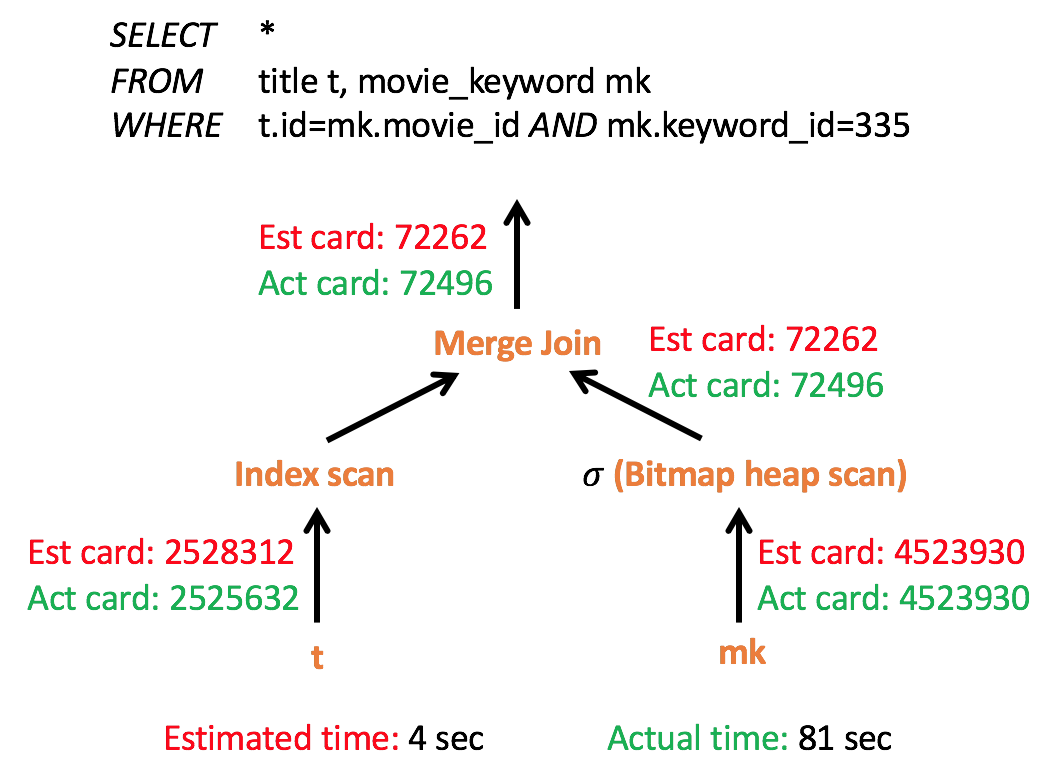
\includegraphics[scale=0.45]{./figs/1a.png}
			\captionof{figure}{Prediction by PostgreSQL without tuned parameters}
			\label{fig:query1}
		\end{subfigure}
	\begin{subfigure}{.5\linewidth}
		\centering
		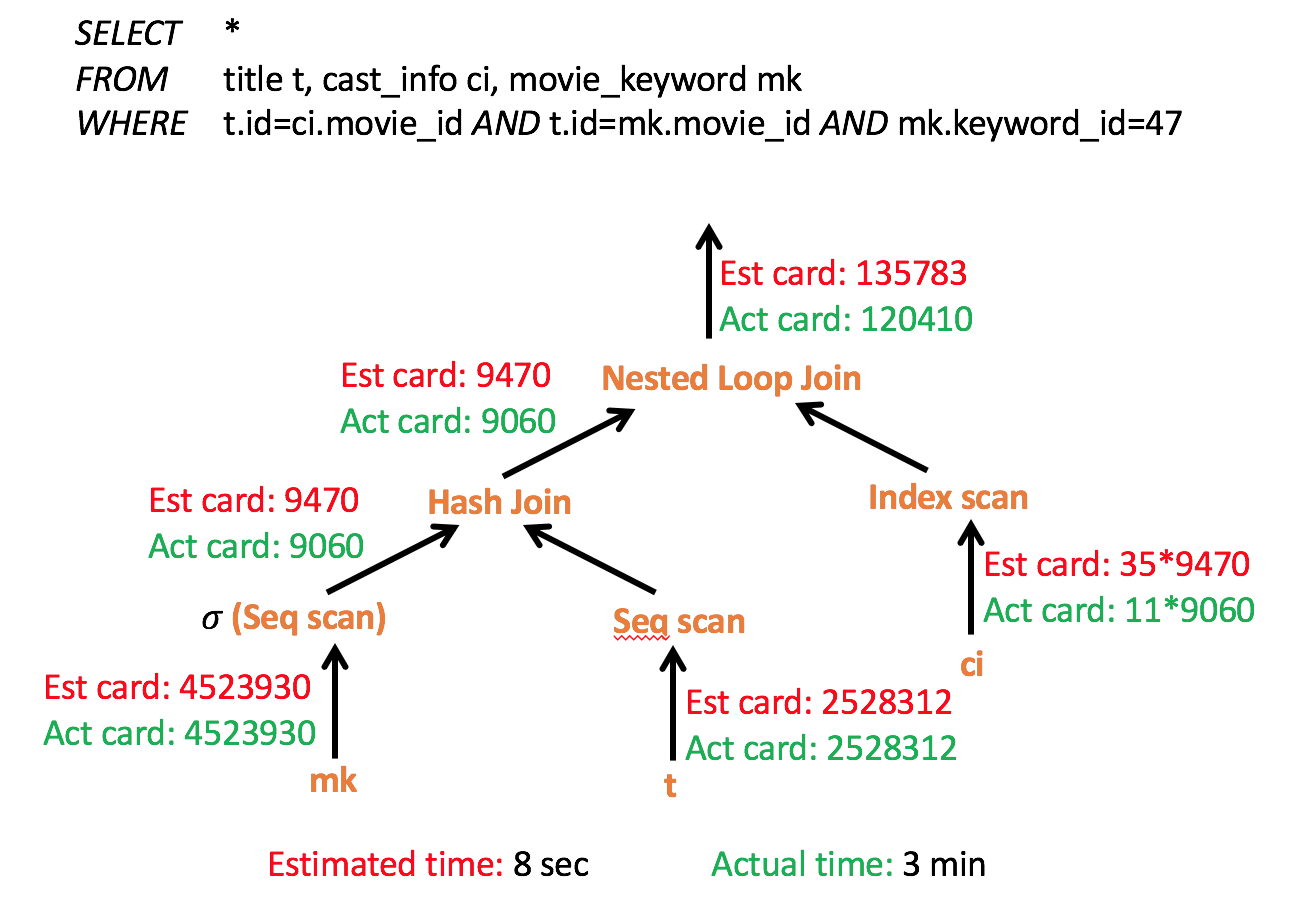
\includegraphics[scale=0.38]{./figs/1b.png}
		\captionof{figure}{Prediction by PostgreSQL with tuned parameters}
		\label{fig:query2}
	\end{subfigure}
	\caption{Example Query Plans}
	\end{figure}


	\begin{figure}
		\begin{subfigure}{\linewidth}
		\centering
		\begin{boxedminipage}{.63\textwidth}     
				\small{
					{\sf \hspace*{0.05in} SELECT * \\
					\hspace*{0.05in} FROM title t, cast\_info ci, movie\_keyword mk\\
					\hspace*{0.05in} WHERE t.id=ci.movie\_id AND t.id=mk.movie\_id AND mk.keyword\_id=47}
					%\hspace*{0.05in} and S.A $>$= 20 and S.A $<$ 60 \hspace*{0.05in} and \hspace*{0.05in} T.C $>$= 2 and T.C $<$ 3
				}
			\end{boxedminipage}
		\captionof{figure}{SQL Query Q}
		\label{fig:sqlquery2}
	\end{subfigure}
	\begin{subfigure}{.5\linewidth}
		\centering
		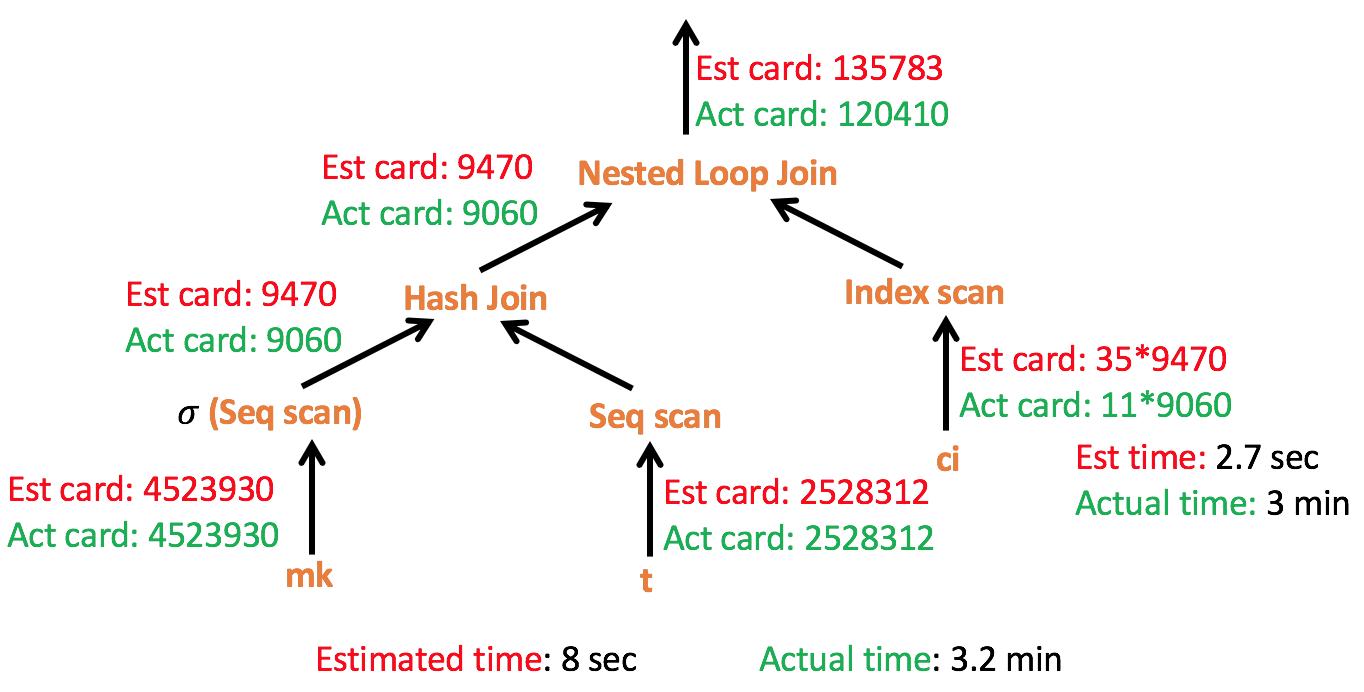
\includegraphics[scale=0.34]{./figs/2a.png}
		\captionof{figure}{Plan A (picked by Wu-tuned Postgres for query Q)}
		\label{fig:query2p1}
	\end{subfigure}
	\begin{subfigure}{.5\linewidth}
		\centering
		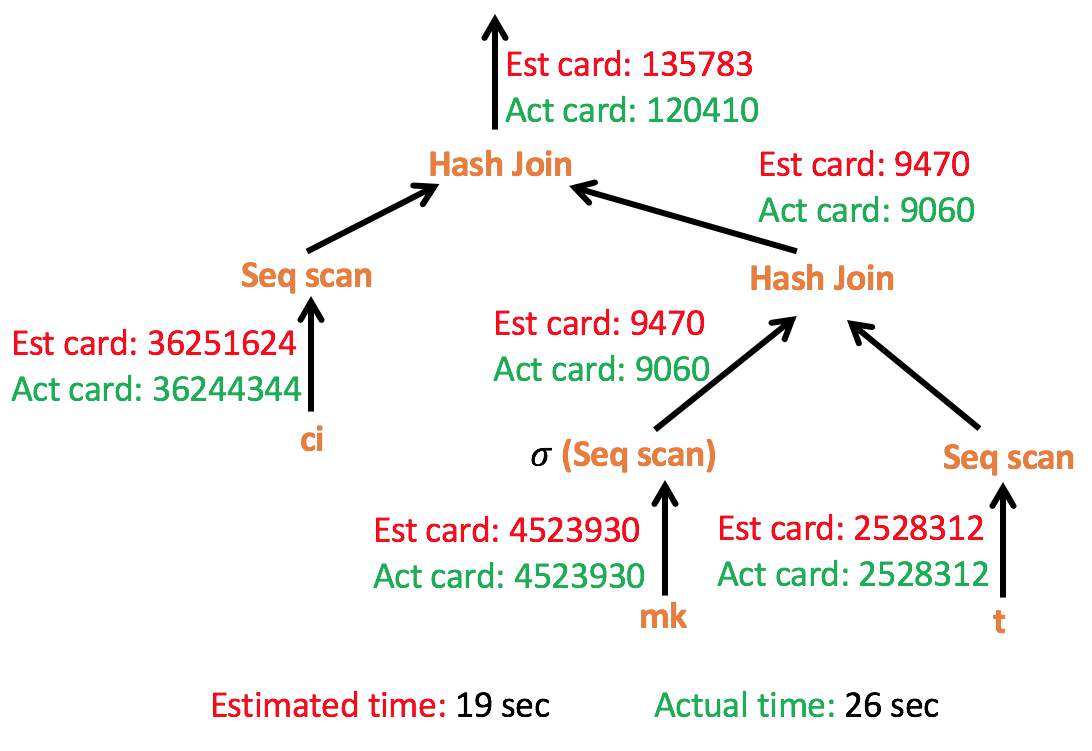
\includegraphics[scale=0.3]{./figs/2b.png}
		\captionof{figure}{Plan B (an alternative better plan for query Q)}
		\label{fig:query2p2}
	\end{subfigure}
	\caption{An example of how bad prediction can affect query optimisation}
	\label{fig:query_op}
\end{figure}

\begin{multicols}{2}
	\section{Prediction of Scan Operators}
	\label{sec:scan}
	We focus only on predicting the scan operators for hard-disk-resident databases. Scan operators typically take up most of the total query execution time (more so in the case of disk-resident databases) and, thus, their prediction is imperative. 
	
	There are two types of scan techniques that DBMSs adopt -- sequential scan and index scan. On running around 20 random queries from Join Order Benchmark (JOB) \cite{job}, we found that 96\% of the total query execution time was spent in scan. Further, 88\% of the total scan time was spent in index scan. 
	
	%In a broad sense, there are two types of scan techniques that DBMSs adopt -- sequential scan and index scan. We ran around 20 queries from Join Order Benchmark (JOB) \cite{job} and found that 96\% of the total query execution time was spent in scan. Further, 88\% of the total scan time was spent in index scan.
	
	%The sequential scan operator reads all the pages of R from the disk sequentially (from the first page to the last page) and returns the tuples qualifying the range [v1,v2]. On the other hand, the index scan operator, assuming an index (often B+ tree) built on the attribute A of relation R, traverses the index from the root to the leaf which contains the value v1 and then traverses from v1 to v2 (stored in sequential order with their respective relation page ids at the leaf level of the index) while reading corresponding data pages from the disk. Index scan is preferred over sequential scan when the number of pages (index+relation) to be read are estimated to be less enough so that the cost of reading few pages (at random locations) would be less than reading the whole relation. Thus, there exists a trade-off between the number of pages (high for sequential scan and low for index scan) and cost of accessing pages (low for sequential scan and high for index scan).

	\begin{center}
		\begin{boxedminipage}{.48\linewidth} 
			\small{
				{\sf \hspace*{0.05in} SELECT * \\
					\hspace*{0.05in} FROM R\\
					\hspace*{0.05in} WHERE v1 $\leq$ A $\leq$ v2}
				%\hspace*{0.05in} and S.A $>$= 20 and S.A $<$ 60 \hspace*{0.05in} and \hspace*{0.05in} T.C $>$= 2 and T.C $<$ 3
			}
			\label{fig:template_q}
		\end{boxedminipage}
		
		\captionof{figure}{Query Template $Q \langle R,A,v1,v2 \rangle $}
		\label{fig:sqlquery3}
	\end{center}


	We will now discuss both the scan operators in detail. For the sake of convenience, let us assume a SQL query $Q \langle R,A,v1,v2 \rangle $ as shown in Figure~\ref{fig:template_q}. Executing Q returns the tuples from relation R whose values of attribute A lie between v1 and v2 (both inclusive). 


	\begin{comment}
	\begin{center}
	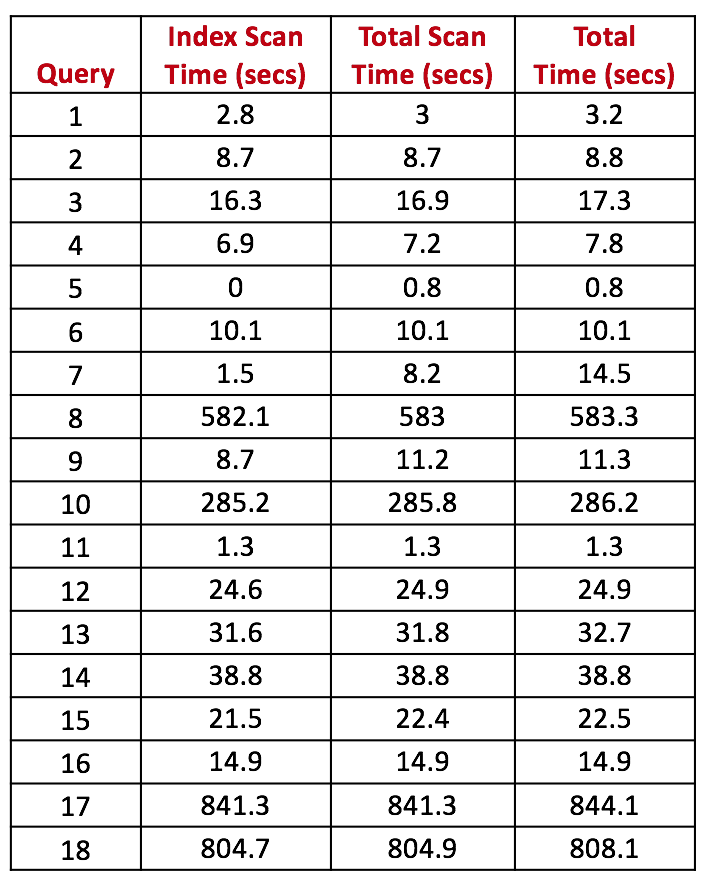
\includegraphics[scale=0.5]{./figs/scanimportance.png}
	\captionof{figure}{IMDB Benchmark Query Execution Time Breakup}
	\label{fig:scanimportance}
	\end{center}
	\end{comment}

	\subsection{Sequential Scan Operator}
	Given a query $Q \langle R,A,v1,v2 \rangle $, PostgreSQL reads the first page (a random access because the disk head can be anywhere initially) and then sequentially accesses the subsequent pages of the relation.
	
	\[Estimated\ Cost = cr + (n-1)*cs\]
	where $n =$ total pages in the relation.
	
	\begin{comment}
	\begin{center}
		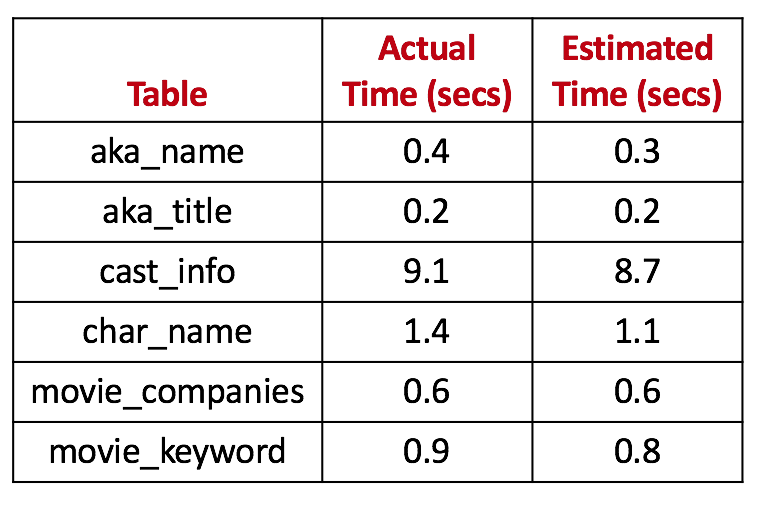
\includegraphics[scale=0.4]{./figs/pg_seq_performance.png}
		\captionof{figure}{PostgreSQL's estimations on Sequential Scan}
		\label{fig:pg_seq_performance}
	\end{center}
	\end{comment}
	
	We evaluated Wu-tuned PostgreSQL optimiser's predictions on all tables in JOB for sequential scan and all the queries were found to have relative error of less than 1\%.
	
	\subsection{Index Scan Operator}	
There can be two types of predicates in a query: equality predicates $(A = v)$ and range predicates $(v1 \leq{A} \leq{v2})$. Currently, we have focused only on range predicates.

During index scan, PostgreSQL first reads the pages of the index from root to the first leaf (containing value $v1$), then reads the data pages corresponding to the values present in that leaf (in order), then reads the next leaf page and repeats the procedure until the relation page with the last value $v2$ has been read. Note that pages once accessed from disk may be found cached next time. Thus, number of disk accesses for data pages are typically not equal to the number of tuples in the range $[v1,v2]$, unless the buffer size is too small. The index stores values of the attribute in ascending order at the leaf level and thus, the data pages can be found at random locations on the disk, unless the index is clustered (i.e. the order of attribute values in index is same as order of attribute values in the relation), in which case index scan simply acts as several partial sequential scans on the table.

\end{multicols}
\newpage
\begin{figure}
	\begin{subfigure}{\linewidth}
		\centering
		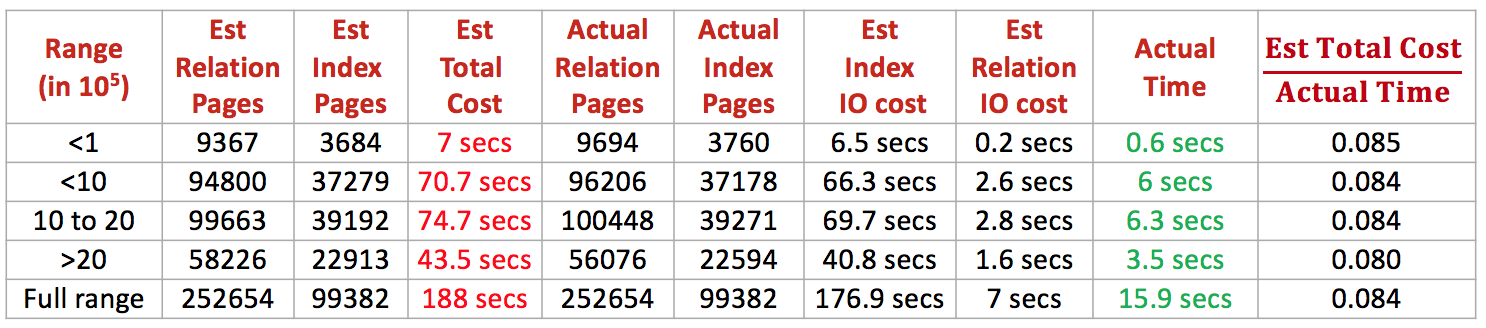
\includegraphics[scale=0.59]{./figs/6a.png}
		\captionof{figure}{$CF = 1: select * from\ cast\_info\_sorted\ where\ v1\leq{movie\_id}\leq{v2}$}
		\label{fig:analysis_corr1}
	\end{subfigure}
	\medskip
	\begin{subfigure}{\linewidth}
		\centering
		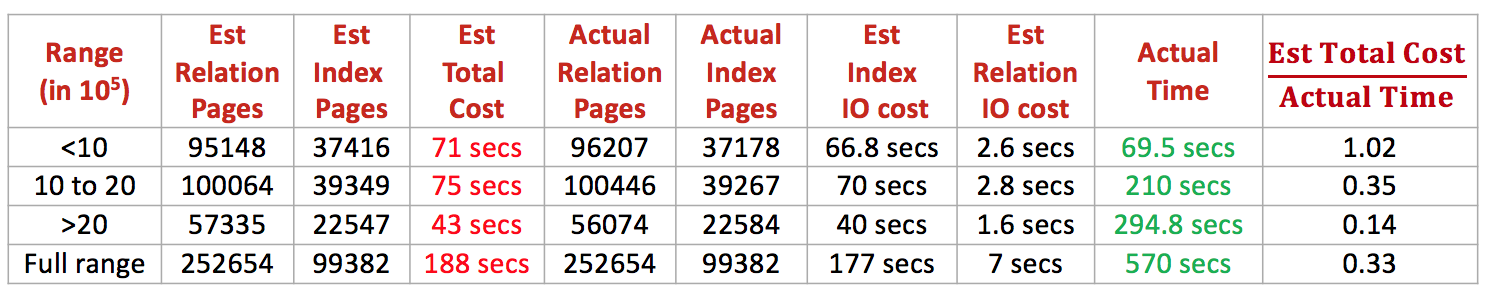
\includegraphics[scale=0.59]{./figs/6b.png}
		\captionof{figure}{$CF = -1: select * from\ cast\_info\_sorted\_desc\ where\ v1\leq{movie\_id}\leq{v2}$}
		\label{fig:analysis_corr_minus1}
	\end{subfigure}
\medskip
\begin{subfigure}{\linewidth}
	\centering
	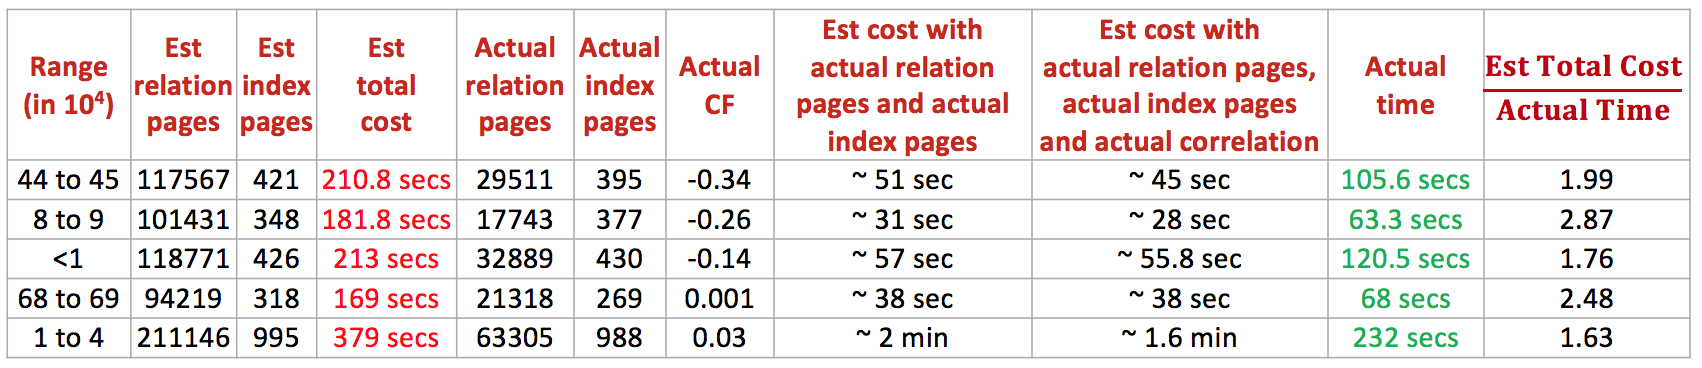
\includegraphics[scale=0.57]{./figs/6c.png}
	\captionof{figure}{$CF = 0: select * from\ cast\_info\ where\ v1\leq{movie\_id}\leq{v2}$}
	\label{fig:analysis_corr0}
\end{subfigure}
	\caption{Experimental analysis of PostgreSQL's cost model for index scan}
	\label{table:pg_index}
\end{figure}
\begin{multicols}{2}
	\section{PostgreSQL's Cost Model of Index Scan}
	\label{sec:cs_index}
	To keep it brief, we have omitted the parts of the model that estimate the time spent in reading index pages from root to leaf, and the CPU cost of processing the index and relation tuples, both of which are negligible compared to the I/O time of the relation pages (interspersed with I/O time of index leaf pages).
	
	For each index on each relation, PostgreSQL maintains a correlation factor $CF$ $\in[-1,1]$ between the attribute values and their respective data page ids, which is essentially a measure of the randomness in the data layout of that particular attribute. $CF = 1$ means the index is clustered (order of attribute values in index being same as order of attribute values in the relation i.e. in ascending order). $CF = -1$ means descending order and $CF = 0$ means maximum randomness in the data layout of the attribute. Using $CF$ value, PostgreSQL interpolates between the minimum $MinC$ (cost of scanning pages sequentially) and maximum cost $MaxC$ (cost of accessing pages from random locations) possible to estimate the cost $C(R)$ of index scan on relation $R$ using the following formula:
	\[C(R) = MaxC + CF^{2}*(MinC - MaxC)\]
	where $MinC$ and $MaxC$ are estimated as follows:
	\begin{equation*}
	\begin{split}
	MinC & = relation\_selectivity * total\_relation\_pages * cs\\
	MaxC & = estimated\_relation\_pages * cr
	\end{split}
	\end{equation*}
	and $estimated\_relation\_pages$ is found by the Mackert and Lohman (M\&L) approximation model \cite{lnm}. 
	\begin{comment}
	which, for a given input ($total\_relation\_pages$, $relation\_selectivity$, $memory\_buffer\_size$), approximates the number of estimated pages to be scanned assuming LRU caching using the following formula :
			$nr = 2 ∗ total_relation_pages ∗ relation_selectivity ∗ \\total_tuples_in_relation / 2 ∗ total_relation_pages\\ + relation_selectivity ∗ total_tuples_in_relation)$
	\end{comment}
	Further, estimated cost to read index pages expressed as $C(I)$ is given as:
	\[C(I) = relation\_selectivity * total\_index\_pages * cr\]
	
	Thus, total cost ($TC$) to read index and relation pages is given as:
	\[TC = C(R) + C(I)\]
	
	%Further, we have assumed the main memory to be big enough to hold all the pages accessed at least once.
	
	\subsection*{Shortcomings in cost modeling}
	
	The above cost model for index scan suffers from following critical limitations:
	\begin{enumerate}
		\item It treats all ranges equally by considering global parameters like $CF$ and $cr$ which could be quite different in the local range of the given query.
		\item It does not distinguish between the positive and negative $CF$ values, whereas the expected behaviour for both cases is different due to rotation of hard disk in a single direction.
		\item  The M\&L formula (to take caching into effect) also does not work well, as shown in experiments below.
		\item The cost model for index scan itself is questionable as it gives inaccurate estimations even after fixing all the above input parameters correctly.
	\end{enumerate}

	To highlight the above shortcomings, we conducted a few experiments on tables with different data layouts.
	\paragraph{Experimental Setup:}
	
	We selected $cast\_info$ table (6.4 GB) from the IMDB dataset and built an index (776 MB) on the attribute $movie\_id$ ($CF \approx 0$). We also created a copy of the relation called $cast\_info\_sorted$ with $movie\_id$ sorted in ascending order ($CF = 1$) and $cast\_info\_sorted\_desc$ with $movie\_id$ sorted in descending order ($CF = -1$).
	
	To take care of perfect cardinality estimate inputs, the metadata statistics parameters were tuned appropriately so that any errors incurred in estimated cost due to cardinality estimation made a difference of at most one second in all the experiments.
	
	\paragraph{Errors due to global parameters:} Figure~\ref{fig:analysis_corr1} shows execution statistics of a few queries for $CF = 1$ case. As we can see from the table, PostgreSQL estimated the relation pages and index pages close to accurate and yet, the estimated times are quite far from the actual execution times. Further, since it is a clustered index case, the global and local $CF$ values are the same. As the index scan here effectively converts to sequential scan (interspersed with index leaf page accesses), the relation scan cost ($MinC$ in this case) was estimated fine but the index scan cost was heavily over-estimated. Since number of index pages were estimated correctly, the problem was in using the global $cr$ value here. Note that the estimated total cost vs actual time ratio is nearly same for all queries and thus, a global but right value of $cr$ can still get estimations right here, as we would expect. However, a $cr$ value favourable to one table/index may not be suitable for another.
		
	\paragraph{Errors due to neglecting sign of $CF$:} Figure~\ref{fig:analysis_corr1} and Figure~\ref{fig:analysis_corr_minus1} show performance of PostgreSQL for $CF = 1$ and $CF = -1$ cases respectively. From the last four rows of the tables we can see that the estimated query execution time is identical while the actual times vary drastically. This is expected since the cost function does not take sign of $CF$ into consideration.
	%Figure~\ref{fig:analysis_corr_minus1} (that shows execution statistics of a few queries of type $Q \langle cast\_info\_sorted\_desc,movie\_id,v1,v2 \rangle $) is an example of PostgreSQL underestimating the cost of index scan, as opposed to other $CF$ cases. Note that the full table scan here took $570$ secs whereas in $CF = 1$ case, it took only 16 secs but PostgreSQL estimated $188$ secs for both. This is because PostgreSQL treats the negative and positive $CF$ values equally. Furthermore, just like in $CF = 1$ case, PostgreSQL estimated relation and index pages fine here but it multiplied $cs$ with estimated relation pages and $cr$ with estimated index pages to get their respective costs, both of which are questionable (former because it's possible that the data pages are not actually stored next to each other and latter because of its value(like in $CF = 1$ case)). It is hard to know what should be the right cost parameters to multiply because the data layout of both index and relation pages is unknown, and thus, as shown in the experiment, estimations can go easily wrong if a particular data layout is assumed.
	
	\paragraph{Errors due to M\&L formula:} As we can see from Figure~\ref{fig:analysis_corr0} i.e. $CF = 0$ case, PostgreSQL overestimated the relation pages using the M\&L formula, making the use of M\&L formula questionable.\\
	
	\paragraph{Erroneous Model Design:} 
	We can see from Figure~\ref{fig:analysis_corr0} ($CF = 0$ case) that even after replacing incorrectly estimated values of the model parameters, i.e. the number of relation pages, index pages and $CF$ with the correct values, the estimated times using the cost model are far from the actual times. This suggests that other than the errors in the estimation of the above three parameters, the model design itself is erroneous. Further, if we take the ratio of estimated time (with the correct input parameters) to the actual time, we do not get a constant implying that a simple constant multiplication factor with the estimated time can also not fix these errors.%  (execution statistics of a few queries of type $Q \langle cast\_info,movie\_id,v1,v2 \rangle $), PostgreSQL nearly correctly estimated the index pages but overestimated the relation pages. But since the local $CF$ values are different from the global $CF (\approx 0$) value, the local $cr$ value (which is dependent on correlation factor) should also be different for each query. However, even if you fix the estimated relation pages and $CF$ value for each query, the estimations are still incorrect rendering the whole model questionable.
	%Note that the ratios of estimated cost and actual time in Figure~\ref{fig:analysis_corr_minus1} and Figure~\ref{fig:analysis_corr0} are uneven and thus, it is not possible to multiply a magic number with PostgreSQL's estimations to get the predictions right.
		
	%In a nutshell, it's not just the aforementioned three major shorcomings in PostgreSQL's cost model that affect its estimations for index scan, the whole model is questionable because, as seen in $CF = 1$, even putting the right values of all parameters gave wrong estimates for queries. 
		\section{Polynomial Regression}
	\label{sec:poly}
	To build a better cost model, it is important to make no assumptions on the data layout. It is expected that if the execution times of all $Q \langle R,A,c,v2 \rangle $-type queries ($c$ is a constant) were plotted on a graph (with cardinality of $[c,v2]$ on x-axis and execution times on y-axis), the curve would be monotonically increasing and look like a series of line segments with different (positive) slopes connected end-to-end, irrespective of the data layout. Furthermore, as the number of pages being cached increase towards the end, most of the new requests would be for already cached pages. Hence, the curve is speculated to have an effectively decreasing slope.
	
\end{multicols}
%\newpage
\begin{figure}
	\label{fig:c1}
\begin{subfigure}{.5\linewidth}
	\hspace{-2em}
	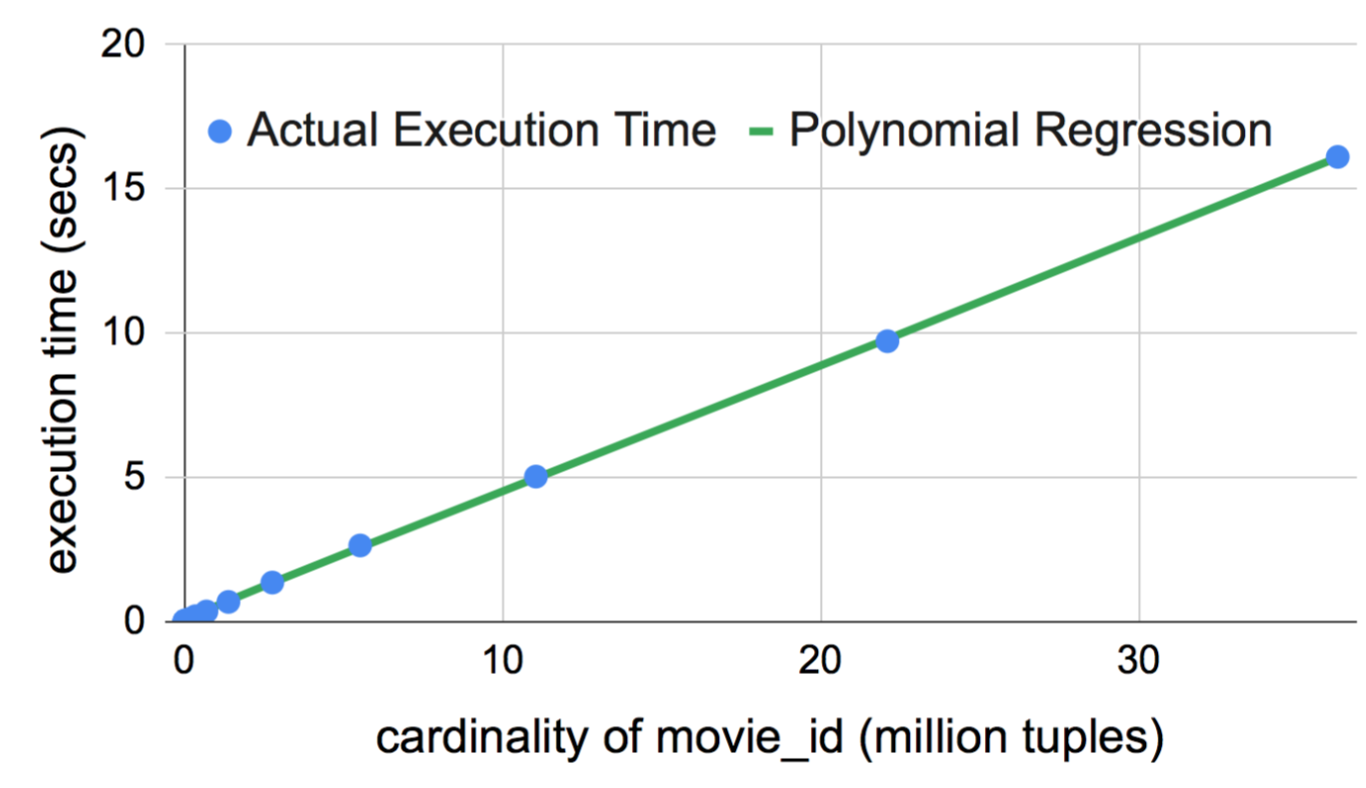
\includegraphics[scale=0.39]{./figs/exp/7/a.png}
	\captionof{figure}{Trained model for $CF = 1$}
	\label{fig:corr1_train}
\end{subfigure}
~
\begin{subfigure}{.5\linewidth}
	%	\centering
	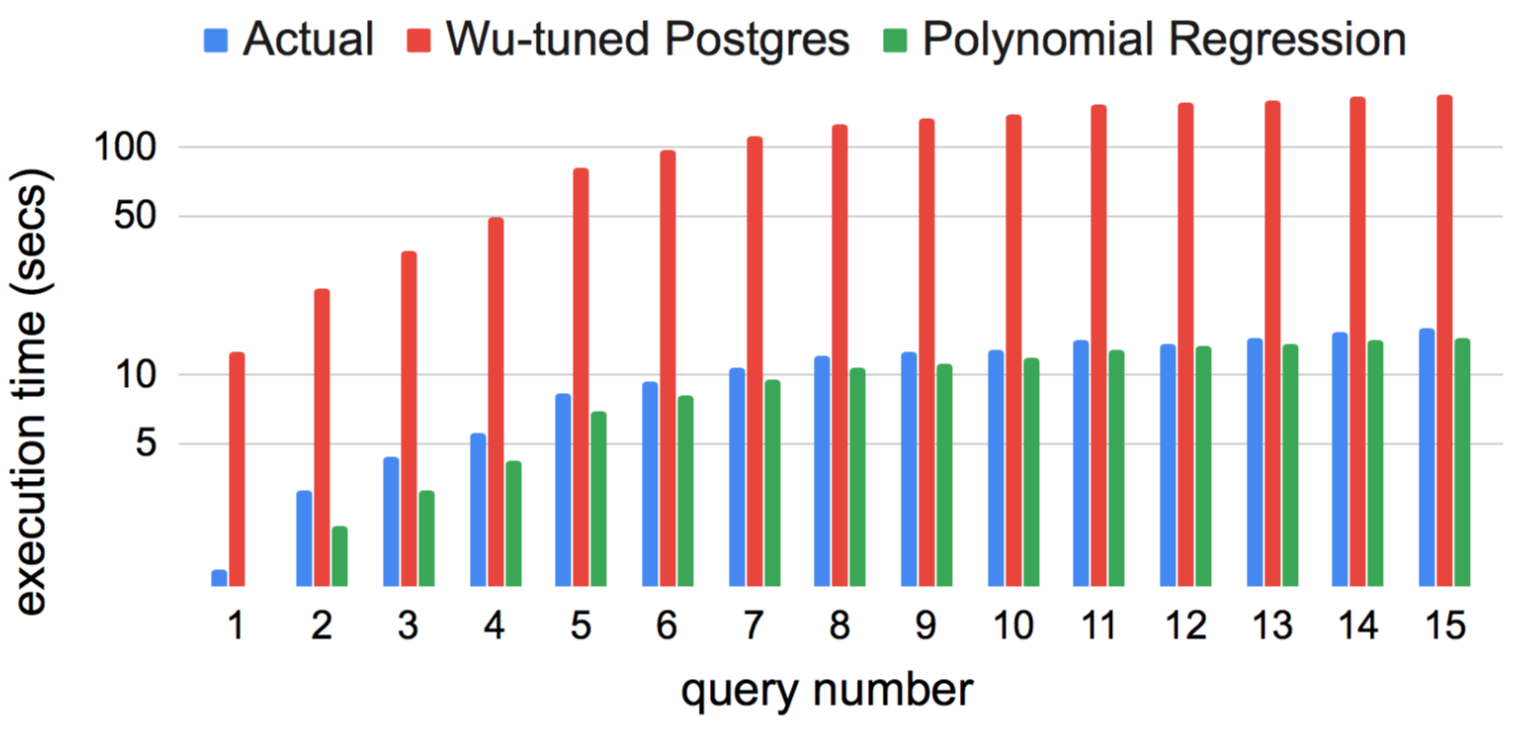
\includegraphics[scale=0.37]{./figs/exp/8/a.png}
	\captionof{figure}{Prediction on test queries for $CF = 1$}
	\label{fig:corr1_test}
\end{subfigure}
\medskip
\begin{subfigure}{.5\linewidth}
	\hspace{-2em}
	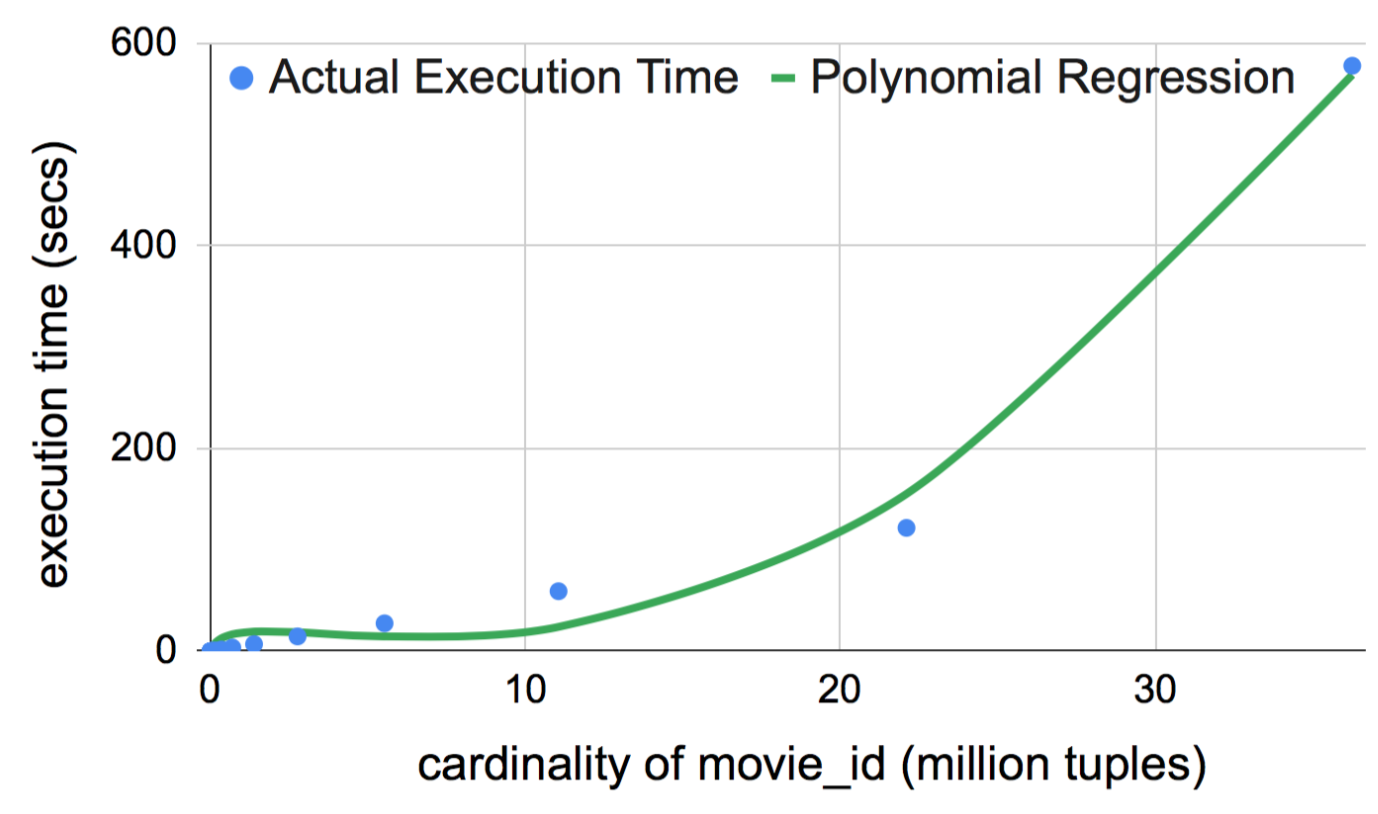
\includegraphics[scale=0.39]{./figs/exp/7/b.png}
	\captionof{figure}{Trained model for $CF = -1$}
	\label{fig:corrminus1_train}
\end{subfigure}
~
\begin{subfigure}{.5\linewidth}
	%\hspace{-2em}
	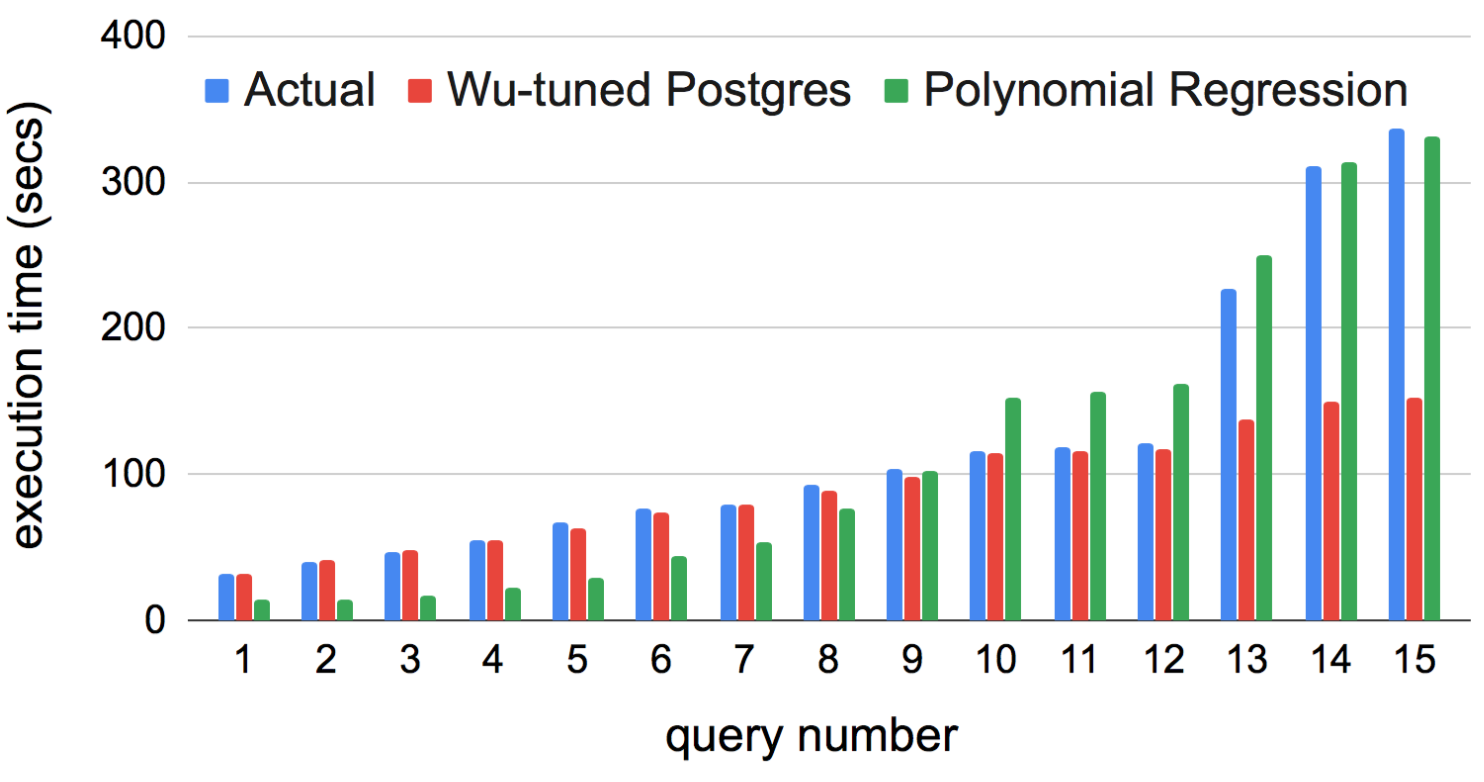
\includegraphics[scale=0.37]{./figs/exp/8/b.png}
	\captionof{figure}{Prediction on test queries for $CF = -1$}
	\label{fig:corrminus1_test}
\end{subfigure}
\medskip
\begin{subfigure}{.5\linewidth}
	\hspace{-2em}
	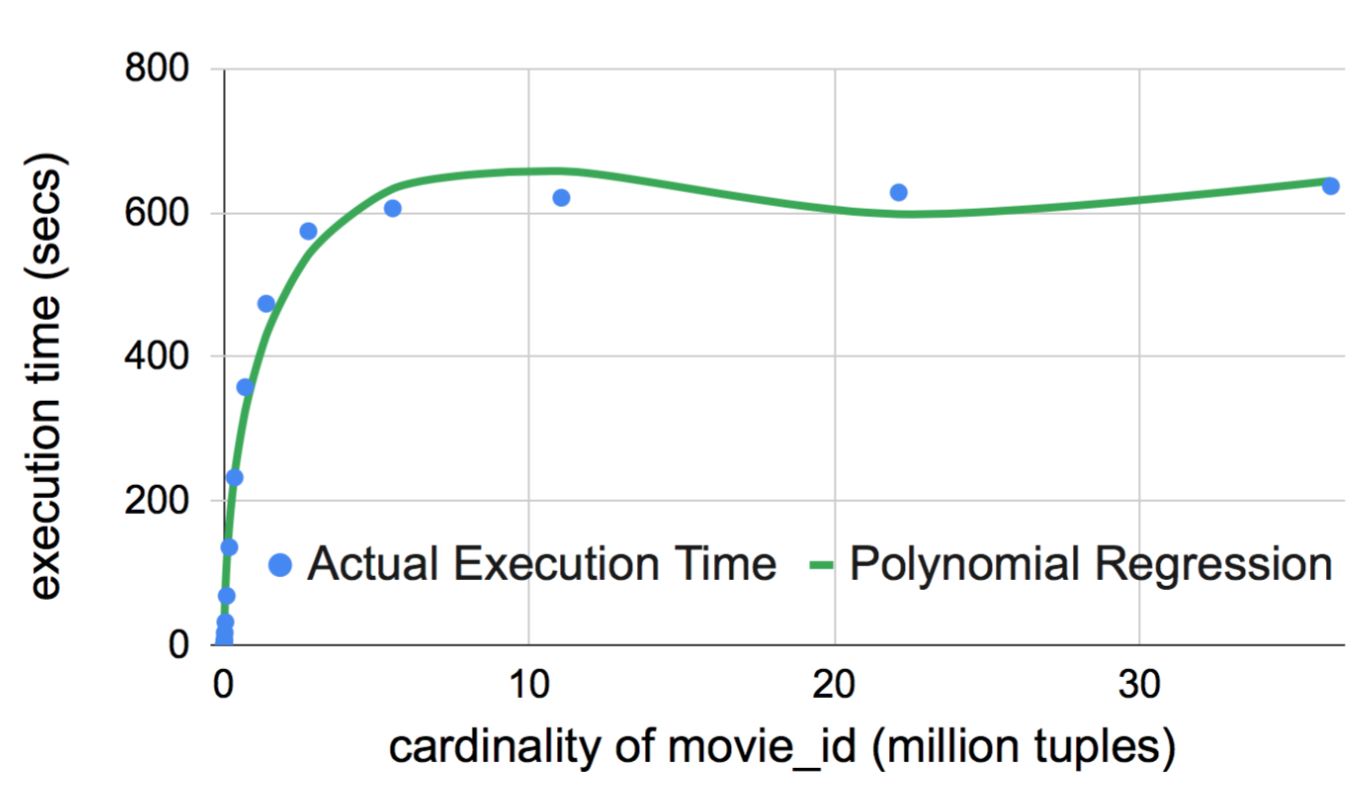
\includegraphics[scale=0.39]{./figs/exp/7/c.png}
	\captionof{figure}{Trained model for $CF = 0$}
	\label{fig:corr0_train}
\end{subfigure}
~
\begin{subfigure}{.5\linewidth}
%	\centering
	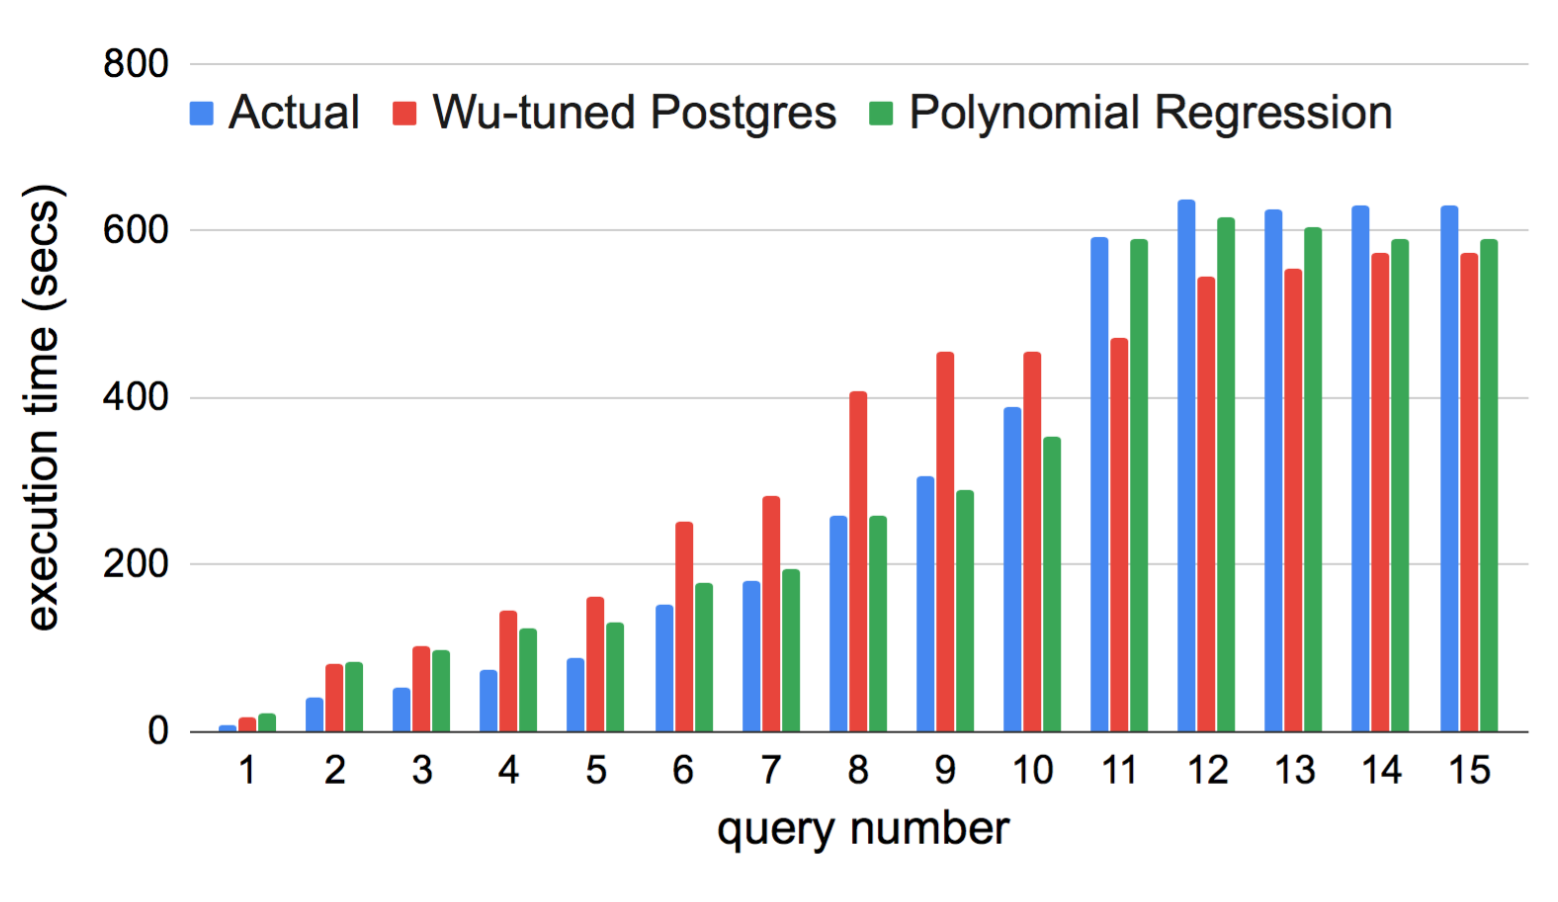
\includegraphics[scale=0.36]{./figs/exp/8/c.png}
	\captionof{figure}{Prediction on test queries for $CF = 0$}
	\label{fig:corr0_test}
\end{subfigure}
\caption{Trained models on different CF values and their predictions on $Q \langle R,movie_id,1,v2 \rangle $-type test queries}
\label{index_performance}
\end{figure}
\newpage
\begin{multicols}{2}
	
Thus, for starters, we have decided to fit a polynomial regressor for $Q \langle R,A,c,v2 \rangle $-type queries.
\section{Experiments}
\label{sec:experiments}
We have run the experiments for $c = 1$ case for $Q \langle R,movie_id,c,v2 \rangle $-type queries where $R = cast\_info/cast\_info\_sorted/cast\_info\_sorted\_desc$. The memory buffers were kept large enough to avoid page replacement. The polynomial regressor was trained on a training data of $log_{2}n$ queries ($n =$ total tuples in the relation) for all the three tables. The $log_{2}n$ training queries are over a geometric sequence of cardinality values with common ratio 2. This way, out of possible 3.5 million (total tuples in $cast\_info$) training queries, only 22 training queries are required. Thus, the training time was very less (a few minutes in total for three indexes), space required to keep the models is O(1) and the prediction time is O(1). The polynomial regressor was chosen to be of the form
\[y_{prediction} = w_{1}*x^{0.5} + w_{2}*x + w_{3}*x^2\]
where $x = $ cardinality in range $[1,v2]$.

For the three tables, the training curves are shown in Figures \ref{fig:corr1_train}, \ref{fig:corrminus1_train} and \ref{fig:corr0_train} and their respective predictions are shown in Figures \ref{fig:corr1_test}, \ref{fig:corrminus1_test} and \ref{fig:corr0_test} respectively. The test queries were picked randomly. As we can see, even a simple ML model (polynomial regressor) trained on very few queries is doing better than the PostgreSQL's model with a mean q-error of 1.2, 1.13 and 1.17 against PostgreSQL's 9.8, 1.96 and 1.36 for $CF = 1, -1$ and $0$ respectively. Note that the models were tested on around 30 queries in each case but only 15 (random) have been shown here due to space constraints. %Training similarly on all values for $v1$ to be able to predict all $Q \langle R,movie_id,v1,v2 \rangle $-type queries, 3.5 million models would have to be trained on $cast\_info$ table. 
\end{multicols}
\begin{figure}[h]
	\begin{subfigure}{.5\linewidth}
		\hspace{-2em}
		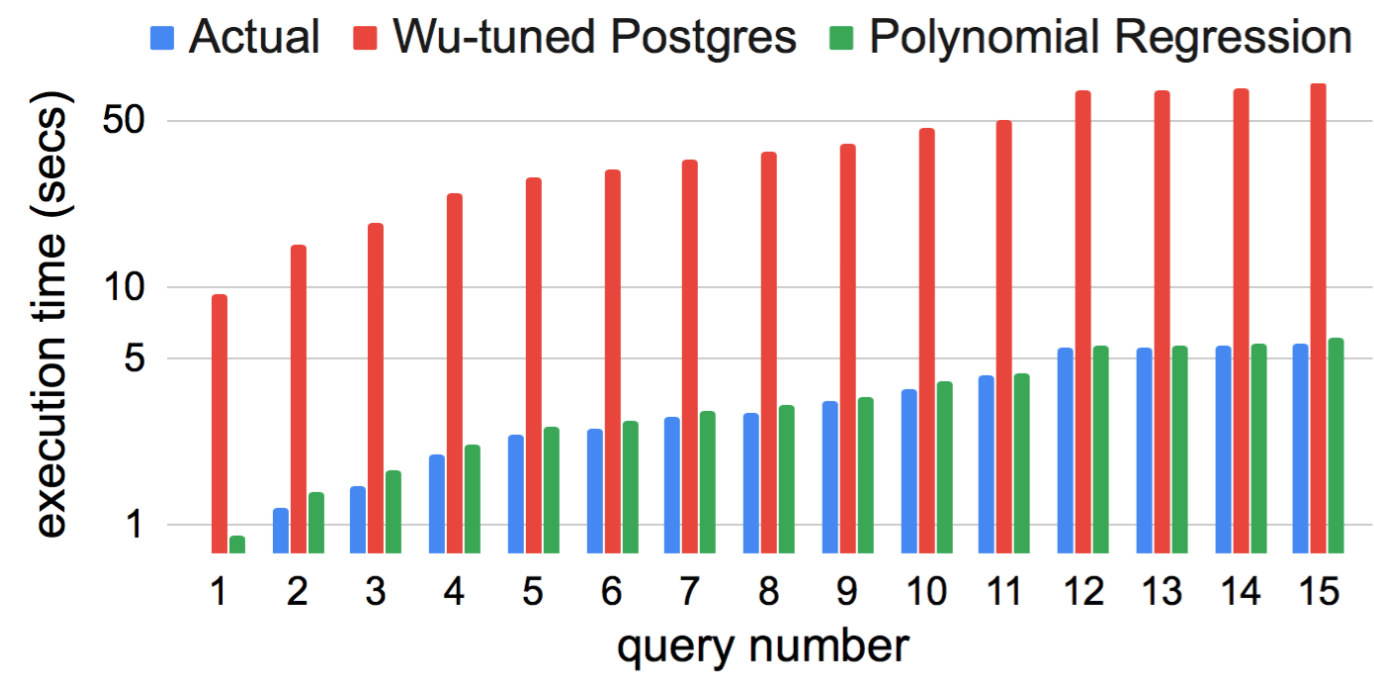
\includegraphics[scale=0.37]{./figs/exp/9/a.png}
		\captionof{figure}{Prediction on test queries for $CF = 1$}
		\label{fig:corr1}
	\end{subfigure}
	~
	\begin{subfigure}{.5\linewidth}
		%	\centering
		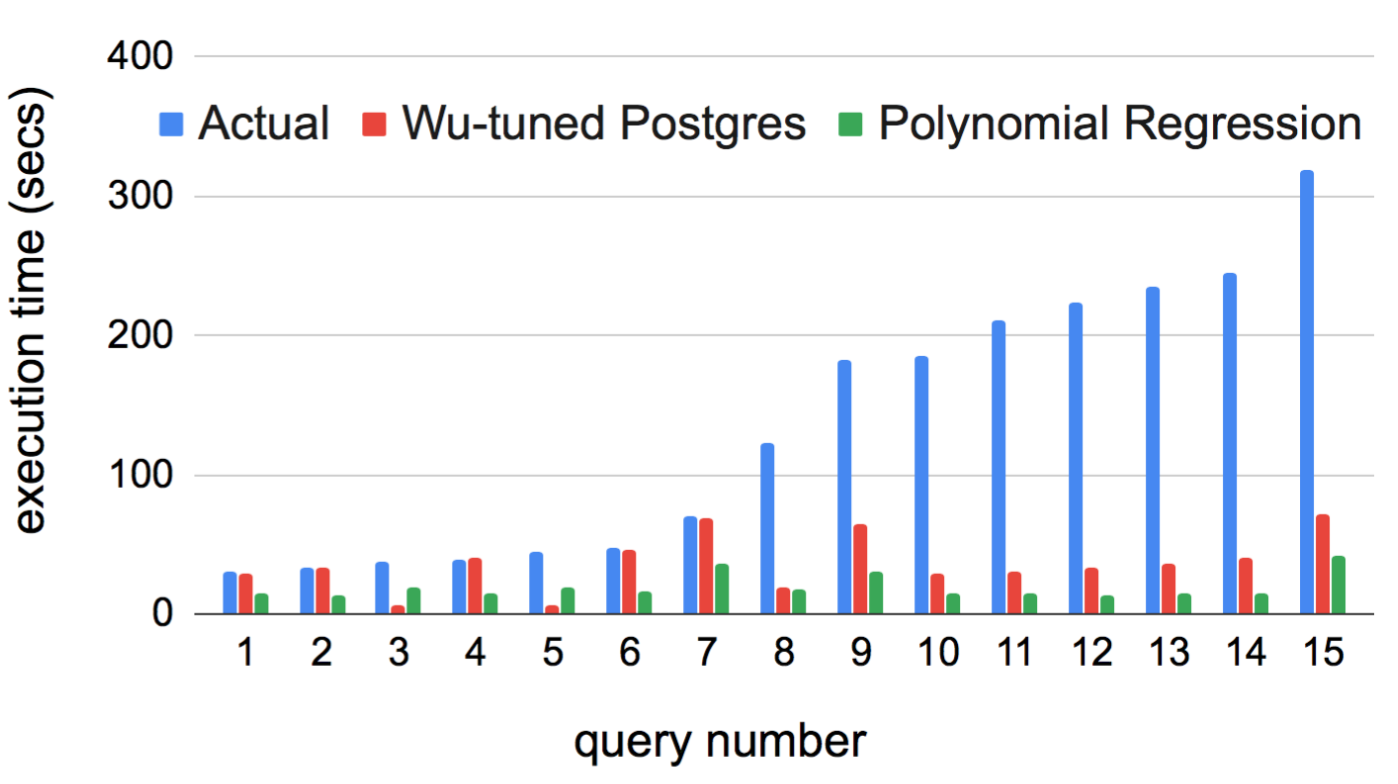
\includegraphics[scale=0.37]{./figs/exp/9/b.png}
		\captionof{figure}{Prediction on test queries for $CF = -1$}
		\label{fig:corr1}
	\end{subfigure}
	\medskip
	\begin{subfigure}{\linewidth}
		\centering
		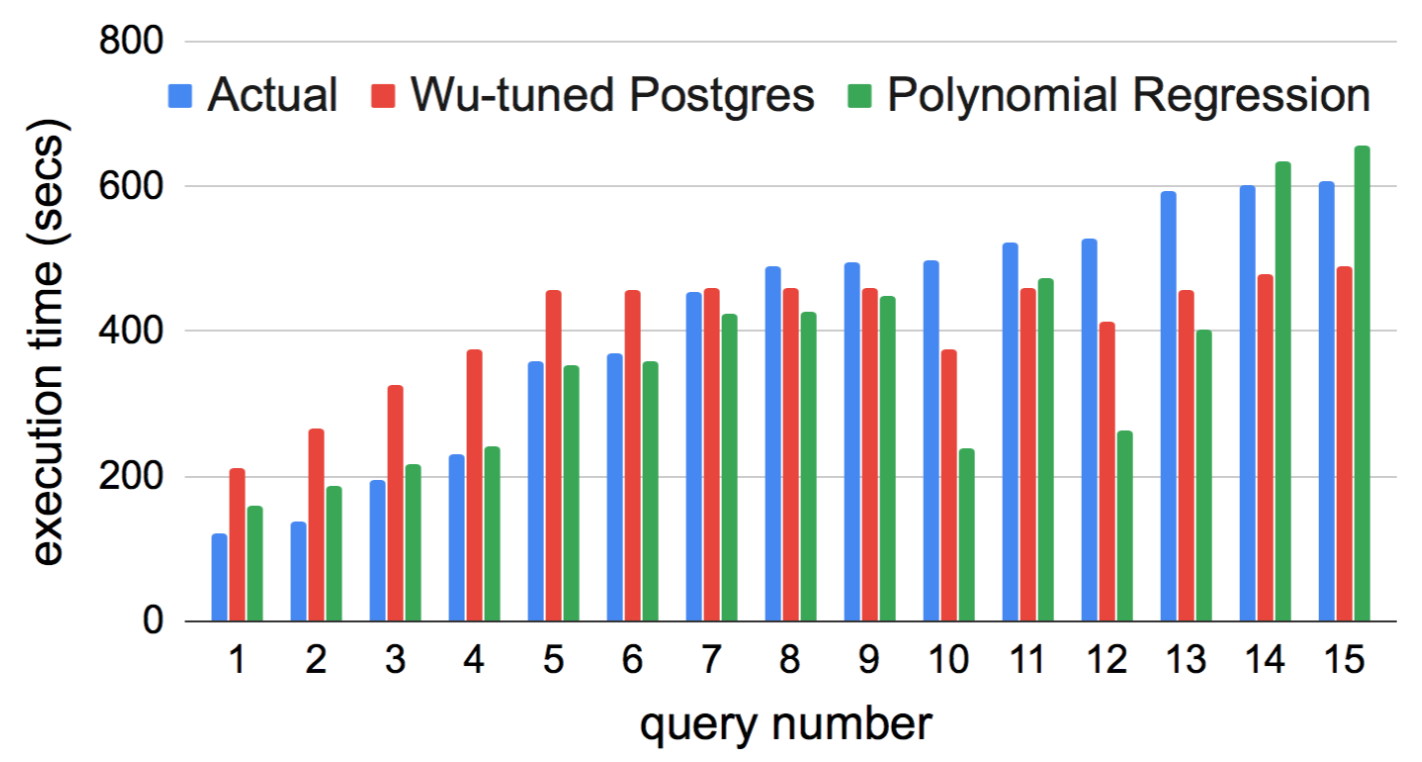
\includegraphics[scale=0.37]{./figs/exp/9/c.png}
		\captionof{figure}{Prediction on test queries for $CF = 0$}
		\label{fig:corrminus1}
	\end{subfigure}
	\caption{Using models in Figure 5 to predict times of $Q \langle R,movie\_id,v1,v2 \rangle $-type test queries}
	\label{fig:range}
\end{figure}
\newpage
\begin{multicols}{2}
	Further, we also did experiments to check if the same model can be used for different values for $v1$, i.e. to inspect if the modeling can be range-location-agnostic (in other words can we predict same time for $[v1,v2]$ or $[v3,v4]$ if both have same cardinality?). To answer this, we used the models created for $v1 = 1$ to answer queries of all values of $v2$ and as expected, the models performed poorly (shown in Figure \ref{fig:range} with q-errors of 1.08, 6.02 and 1.25 respectively). Thus, the models cannot be range-location-agnostic. A possible way to tackle this problem is to bucketise the whole range of cardinality into k buckets and use the same model for each bucket. This is because, for instance, a model for $Q \langle R,movie_id,1,v2 \rangle $ and $Q \langle R,movie_id,2,v2 \rangle $ should not be much different. But, the challenge is how to bucketise the whole range so that the training time is less, the space required to store the model is less and the prediction time is less.
	\section{Related Work}
	\label{sec:relwork}
	Wu et al. followed their statistical tuning \cite{wu} approach by trying to tackle the noise in the cost tuning parameters \cite{wu_wu}. As part of ML-based research, Chetan et al. \cite{chetan} used random forest technique on an ensemble of models (like k-nearest neighbour) to give a band of execution time. Ganapathi et al. \cite{ganapathi} took plan-level features of a query plan and applied a Kernel Canonical Correlation Analysis (KCCA) approach to predict not just time but other metrics like CPU usage, memory usage, etc. Akdere et al. \cite{akdere} went for a hybrid modeling approach by using SVM at plan level and linear regression at operator level. Li et al. \cite{surajit} applied linear regression on all the nodes of a plan and scaled the results at runtime to get better estimates. Finally, there has been recent work \cite{marcus} that learns a neural network model for each operator and combines the result using another neural network on top.
	
	\section{Conclusions and Future Work}
	\label{sec:conclusions}
	In conclusion, the cost model of PostgreSQL for index scan does not seem to provide good estimations and it seems possible to leverage the data layout to build a simple and explainable machine learning model which can do better predictions. The next step is to see if fitting piece-wise curve on better training data can improve predictions. Then, the next step is to see how to handle all $Q \langle R,movie_id,v1,v2 \rangle $-type queries then head on to handle the equality predicates. After that, other scan operators like bitmap heap scan and internal node operators like join and aggregate need to be looked at. Uncertainties like spilling are also a part of the future aspects of the project.
	
    \bibliographystyle{abbrv}
\begin{thebibliography}{10}
	
	\bibitem{akdere}
	M.~Akdere and U.~{\c C}etintemel.
	\newblock Learning-based Query Performance Modeling and Prediction.
	\newblock In {\em ICDE}, 2012.
	
	\bibitem{ganapathi}
	A.~Ganapathi, H.~Kuno, U.~Dayal, J. L. ~Wiener, A. ~Fox, M. ~Jordan and D. ~Patterson.
	\newblock Predicting Multiple Metrics for Queries: Better Decisions Enabled by Machine Learning.
	\newblock In {\em ICDE}, 2009.
	
	\bibitem{chetan}
	C.~Gupta, A.~Mehta, and U.~Dayal.
	\newblock PQR: Predicting Query Execution Times for Autonomous Workload Management.
	\newblock In {\em ICAM}, 2008.
	
	\bibitem{job}
	V.~Leis, A.~Gubichev, A.~Mirchev, P.~Boncz, A.~Kemper and T. Neumann.
	\newblock How Good Are Query Optimizers Really?
	\newblock {\em PVLDB}, 9(3), 2015.
	
	\bibitem{surajit}
	J.~Li, A. C~K{\"o}nig, V.~Narasayya, and S.~Chaudhary.
	\newblock Robust Estimation of Resource Consumption for SQL Queries using Statistical Techniques.
	\newblock {\em PVLDB}, 5(11), 2012.
	
	\bibitem{marcus}
	R. Marcus and O. Papaemmanouil.
	\newblock Plan-Structured Deep Neural Network Models for Query Performance Prediction.
	\newblock In {arXiv}, 2019.
	
	\bibitem{lnm}
	L. F.~Mackert and G. M.~Lohman.
	\newblock Index Scans Using a Finite LRU Buffer: A Validated I/O Model.
	\newblock {\em TODS}, 14(3), 1989.
	
	\bibitem{wu}
	W.~Wu, Y.~Chi, S.~Zhu, J.~Tatemura, H.~Hacig{\"u}m{\"u}s and J. F.~Naughton.
	\newblock Predicting Query Execution Time: Are Optimizer Cost Models Really Unusable?
	\newblock In {\em ICDE}, 2013.
	
	\bibitem{wu_wu}
	W.~Wu, Xi~Wu, H.~Hacig{\"u}m{\"u}s and J. F.~Naughton.
	\newblock Uncertainty Aware Query Execution Time Prediction.
	\newblock {\em PVLDB}, 7(14), 2014.
	
\end{thebibliography}

	\end{multicols}
\end{document}
